\section{Obstructed Leaves} \label{sec:leaves}

Suppose that some clique-point $a$ cannot be placed, so $\da_a = \emptyset$.  In terms of
$\wlt$, we get $a \wlt a$. Since $\wlt$ is a strict partial ordering, this already makes the partial
representation non-extendible.

\begin{lemma}[The leaf case] \label{lem:leaf}
If a leaf is obstructed, then $G$ and $\calR'$ contain an SE, or 1-BI obstruction.
\end{lemma}

\begin{proof}
We name the vertices as in the definition of the 1-BI obstructions. Suppose that the leaf corresponds
to a maximal clique $a$ such that $\da_a = \emptyset$.  

Let $u \in P^{\endlft}(a)$ and $v \in P^{\startrt}(a)$ (possibly $u = v$). Since $I_a$ is a
subinterval of $\bigcap_{w \in P(a)} \inter w'$ and $\da_a = \emptyset$, every point of
$[\ell(v),r(u)]$ is covered by some pre-drawn interval not contained in $P(a)$. Let $\inter{x_1}'$
be one such interval covering $\ell(v)$ and let $\inter{z_1}'$ be one such interval covering $r(u)$
(again, possibly $x_1=z_1$); see Fig.~\ref{fig:leaf}. Let $P_1$ be a shortest path from $x_1$ to
$z_1$ consisting of pre-drawn intervals not in $P(a)$.

\begin{figure}[t!]
\centering
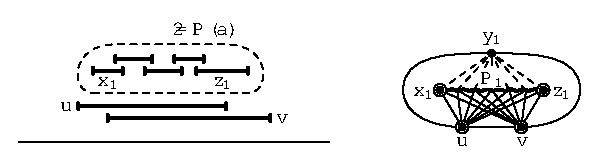
\includegraphics{leaves_construction_of_1-BI.eps}
\caption{A construction leading to a 1-BI obstruction.}
\label{fig:leaf}
\end{figure}

We prove that the relative pre-drawn position of $u$, $v$, $x_1$, and $z_1$ makes the partial
representation non-extendible. The maximal clique $a$ does not contain any vertex of $P_1$.  Since
the vertices of $P_1$ induce a connected subgraph, by Lemma~\ref{lem:non_adjacent} there exists $y_1
\in a$ which is non-adjacent to all vertices of $P_1$.  Hence, these (at most) five vertices
together with $P_1$ create either a 1-BI obstruction (when $\ell(u) < r(v)$), or an SE obstruction
(when $\ell(u)=r(v)$, for which $x = x_1 = z_1$ and we can free it). We note that this obstruction might not be minimal,
in which case we can remove some vertices and get one of the minimal obstructions illustrated
in Fig.~\ref{fig:SE} and~\ref{fig:BI_obstructions}.\qed
\end{proof}

